\chapter{The Automated Executions Plug-in}
This chapter describes the Automated Execution plug-in that is responsible for handling
the setup, control flow and display of an automated execution run.
Although the plug-in is structured according to the model-view-controller pattern this
is not the structure that this chapter will to describe it. Instead this chapter will
follow the structure already used in the previous chapters. Which means the chapter will
consist of four parts:
\begin{enumerate}
 \item The setup of an automated execution run with a description of the wizard.
 \item The input to the automated execution. This section will describe the newly created interface.
 \item The control flow of the automation with the Automation Job and the Automation Wizard.
 \item The ouput of the automation run. In this section the new view and the results structure will
be described.
\end{enumerate}


\section{Automation Setup - The Wizard}
\label{section:AutoWizard}
\index{Wizard}
As described in Section \ref{section:AutoConceptsSetup} an Eclipse wizard will be used to set up the 
automated run. Automation Wizard consists of two pages:
\begin{enumerate}
 \item The File Selection Page for selecting all files that should be involved in the automated run.
 \item The Property Setting Page for defining custom properties that the components should receive prior to
each iteration.
\end{enumerate}


\subsection{File Selection Page}
\begin{figure}[File Selection Page]
  \centering
  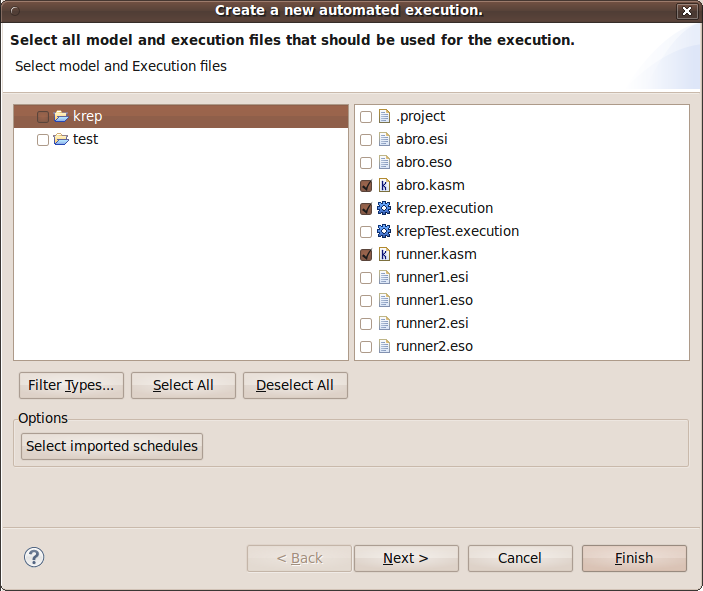
\includegraphics[scale=.4]{FileSelectionPage.png}
  \caption[The Wizard Page for selecting the input files for an automated run.]%
  {The Wizard Page for selecting the input files for an automated run.\protect}
  \label{fig:FileSelectionPage}
\end{figure}
The File Selection Page shown in Figure \ref{fig:FileSelectionPage} is used to select the model 
files and execution files that should be used for the automated run.

Since Eclipse already provides a variety of pre-made wizard pages it can be avoided to write a page for a
complex task like this from scratch. The wizard that can be modified to fit the needs of the task at hand
is the standard Eclipse Resource Import Wizard. It is normally used to select a number of files and folders
for import into the 

- extends ResourceImportWizard for displaying a folder/file structure for selecting files from
- easily usable, select whole folders, filter file types
- can be given an initial selection, on close will save the selection, store it in preference store
and restore it on load
- additional dialog for selecting execution files that are not in the workspace but imported
- for simplicity assume that files ending .execution are execution files and all other selected
ones are model files, wizard can not check if valid since formats are not known
- only allow user to proceed if at least one execution and one model file is selected
\subsection{Property Setting Page}

\begin{figure}[Property Setting Page]
  \centering
  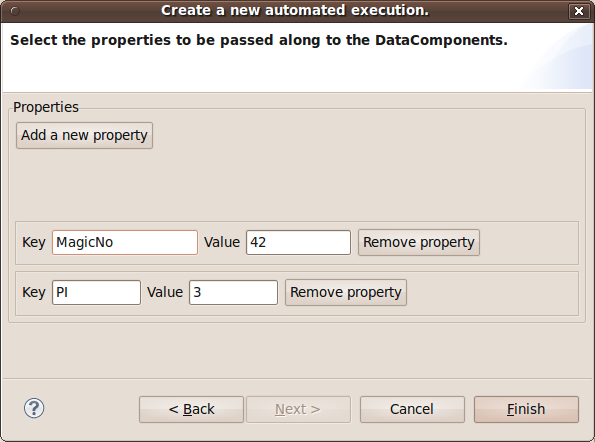
\includegraphics[scale=.4]{PropertySettingPage.png}
  \caption[The Wizard Page for setting up user defined properties.]%
  {The Wizard Page for setting up user defined properties.\protect}
  \label{fig:PropertySettingPage}
\end{figure}
- set up the additional arguments passed to the execution
- simple adding and removing of key, value pairs
- same as file page, on close results are saved to preference store and restored for initial
selection on next open
\subsection{Information Processing}
- gather execution files and model files from file selection page
- gather properties from property page
- store information for next open
- invoke the execution manager


\section{Automation Input}
\label{section:AutoInput}
In order to provide the DataComponents with input prior to each part of the automated run new interfaces
had to be created in order to interact with the components.

\subsection{Automated Component}
An automated component is any DataComponent (see Section \ref{section:IntroDataComponent}) that wants to interact with
the automated execution plug-in. An automated component has to provide the following three methods:

\begin{description}
 \item \textbf{void setParameters(List<KiemProperty> properties) throws KiemInitializationException} : 

This method enables components to receive information prior to each execution
run. The list is implemented as an array of key, value pairs stored inside
KiemProperty objects.
At the every least the list contains the location of the model file and the
index of the currently running iteration.
This allows components to load additional files that are always in the
same path as the execution file and determine which of those to load
based on the iteration index.
The custom properties that the user defined through the wizard for example are
also added here.
If the component encounters an error during at this point because for example a model file
could not be loaded it should respond by throwing the declared Exception.

 \item \textbf{int wantMoreSteps()} : 

This method is called before the Automation Manager performs the first step.
All components will be asked how many steps they are likely to need for their
execution run. The maximum of these values will be taken and the execution
will perform the requested number of steps. After that the components
will be asked again and so on. The process stops when all components
answer with zero.

 \item \textbf{int wantsMoreRuns()} : 

This method works analog to the wantMoreSteps() method in the context
of entire execution runs. It is used to determine how many iterations
should be performed with the given combination of execution file and model
file.
\end{description}

\subsection{Automated Producer}
This interface extends the AutomatedComponent interface.
In addition to the inherited methods it provided one additional method.
This method is called after an iteration has finished and asks the components
if they want to publish any information about the results of their execution.
This information is gathered by the plug-in and the accumulated results
are either passed to the calling plug-in or displayed in the
specially designed view (see Section \ref{section:AutoView}).



\section{Automation manager and Automation Job}
- handles control flow during the automation
- takes information from either call through the API or wizard

\subsection{Automation Manager}
- handles the overall control flow
- takes the execution files, model files and properties as argument
- if progress monitor is registered it is informed about the progress of the evaluation
- The control flow:
\begin{itemize}
 \item iterate over all execution files
 \item open execution file
 \item tell view to set up display for the first execution file
 \item iterate over all model files
 \item get first model file from list
 \item ask components how many more runs they need, take maximum and perform runs before asking again
 \item pass model file, execution file and index of iteration
 \item initialize the execution
 \item pass properties to components, at least receive model file and iteration
 \item start worker thread that listens for monitor canceling, step timing out
 \item ask components how many more steps they need, take maximum and perform steps before asking again
 \item perform one step, lock self inside semaphore, stay locked until either worker thread or event listener notifies (step done)
 \item when no component wants more steps pause
 \item gather information from all IAutomatedProducers
 \item tell view to show information for this iteration
 \item stop execution inside the KIEM and perform cleanup
 \item proceed to next iteration
 \item inform monitor of progress
 \item proceed to next model
 \item proceed to next execution
 \item when done inform monitor of done and terminate the job
\end{itemize}



\subsection{Automation Job}
- workbenchjob with progressmonitor
- used to display the progress in the progress view and a dialog with progress bar
- long running task, doesn't want to block the rest of the workbench 
- triggers execution in the manager

\section{Automation View}
\label{section:AutoView}
- displays the information in a structured way
- start a new table for each execution file
- one row for each iteration with each model file
 - prerequisite needed here: always the same outputs throughout the entire execution file
- first columns display model file name, iteration index and current status

\subsection{Tool bar}
- button to start the wizard
- button for clearing the view
- text field showing the step that was just processed
